\lecture{Estimador de fase}{lec_carrier}

\begin{frame}
	\begin{block}{\centering\large\bfseries Parte 7}
		\centering\large\insertpart
	\end{block}
\end{frame}

\section{Método \(M\)-power}
\begin{frame}[t]
	\frametitle{Método \(M\)-power}
	
	\begin{itemize}
        \item O método \(M\)-\textit{power} consiste em uma técnica de estimação de fase em malha aberta (\textit{feedforward}) para sinais \(M\)-PSK sem offset \footnote{O esquema OQPSK, por exemplo, não se adequa a este método.}.
        \item Este método é NDA (\textit{non-data-aided}), pois não depende dos simbolos transmitidos.
        \item Suporemos que o demodulador possiu perfeito conhecimento do atraso de símbolo, \(\tau\), e do o desvio de frequência, \(\nu\). Sendo assim, trabalharemos apenas com \(\theta\), i.e.,
        \begin{align}
            s(t, \hat{\theta}_{k}) = s_l (t) e^{j\hat{\theta}_{k}}.
            \label{eq:s_t}
        \end{align}
        % Neste cenário, a função de verossimilhança depende de dois termos desconhecidos para o demodulador: os símbolo transmitidos, \(\left\{ A_k \right\}\), e o desvio de fase, \(\theta\). Portanto, denotaremos o critério ML como \(\Lambda(\mathbf{r}_k|\hat{\theta}_{k})\)
        \item O estimador é derivado a partir da suposição de que o sistema opera em uma baixa SNR. Esses cenários tornam os métodos DD ineficientes uma vez que a BER do sistema é maior.
    \end{itemize}
\end{frame}

\begin{frame}[t]
	\frametitle{Método \(M\)-power}
    \begin{itemize}
        \item Do slide anterior, temos que
        \begin{align}
            \Lambda(\mathbf{r}_k|\hat{\theta}_{k}) = \textnormal{exp} \left\{ \frac{2}{K}  \int_{(k-K)T}^{kT} \textnormal{Re}\left\{r(t)s^*(t, \hat{\theta}_{k})\right\} \diff{t} \right. \nonumber \\
            \left. - \frac{1}{K} \int_{(k-K)T}^{kT} \abs{s(t, \hat{\theta}_{k})}^{2} \diff{t} \right\}
            \label{eq:init}
        \end{align}
        \item Recordando que \(\abs{z}^2 = z z^*\), para \(z \in \mathbb{C}\), e que
        \begin{align}
            s_l (t) = \sum_k A_k g(t - kT)
        \end{align}
        \begin{itemize}
            \item \(A_k \in \mathbb{C} \rightarrow\) \(k\)-ésimo śimbolo transmitido
            \item \(g(t) \in \mathbb{R} \rightarrow\) pulso formatador
        \end{itemize}
    \end{itemize}
\end{frame}

\begin{frame}[t]
	\frametitle{Método \(M\)-power}
    \begin{itemize}
        \item podemos reescrever o segundo termo da Eq.\eqref{eq:init} como
        \begin{align}
            \frac{1}{K} \int_{(k-K)T}^{kT} \abs{s(t, \hat{\theta}_{k})}^{2} \diff{t} = \frac{1}{K} \sum_{i = k-K}^{k} \sum_{p = m-K}^{m} A_i A_p^*h\left( \left[ i-p \right]T \right)
            \label{eq:seg-term1}
        \end{align}
        \begin{itemize}
            \item \(h\left( t \right) = g(t) * g(-t) = \int_{-\infty}^{\infty} g(t) g(t - kT) \diff{t}\)
        \end{itemize}
        \item E o primeiro termo como
        \begin{align}
            \frac{2}{K} \int_{(k-K)T}^{kT} \textnormal{Re}\left\{r(t)s^*(t, \hat{\theta}_{k})\right\} \diff{t} = \frac{2}{K} \sum_{i = k-K}^{k} \textnormal{Re} \left\{ x_i A_i^* e^{-j \hat{\theta}_{i}} \right\}
        \end{align}
        \begin{itemize}
            \item \(x_k = \eval{\left[r(t) * g(-t)\right]}{t=kT} \)
        \end{itemize}
    \end{itemize}
\end{frame}

\begin{frame}[t]
	\frametitle{Método \(M\)-power}
	\begin{itemize}
		\item Como \(h\left( t \right)\) obedece o critério de Nyquist e \(z^*z = \abs{z}^2\) para \(z \in \mathbb{C}\) , a equação \eqref{eq:seg-term1} se torna
		\begin{align}
            \frac{1}{K} \int_{(k-K)T}^{kT} \abs{s(t, \hat{\theta}_{k})}^{2} \diff{t} = \frac{1}{K} \sum_{i = k-K}^{k} \abs{A_i}^2
        \end{align}
        \item Substituindo essas concluções, tem-se
        \begin{align}
            \Lambda(\mathbf{r}_k|\hat{\theta}_{k}) = \textnormal{exp}\left\{ \frac{2}{K} \sum_{i = k-K}^{k} \textnormal{Re} \left\{ x_i A_i^* e^{-j \hat{\theta}_{i}} \right\} - \frac{1}{K} \sum_{i = k-K}^{k} \abs{A_i}^2 \right\}
        \end{align}
	\end{itemize}
	
\end{frame}

\begin{frame}[t]
    \frametitle{Método \(M\)-power}

    \begin{itemize}
        \item A equação anterior se torna mais elegante se observarmos que a métrica de decisão \(\Lambda(\mathbf{r}_k|\hat{\theta}_{k})\) pode ser mutiplicada pelo fator
        \begin{align}
            \textnormal{exp}\left\{ - \frac{1}{K} \sum_{i = k-K}^{k} \abs{x_i}^2 \right\}
        \end{align}
        sem causar consequnências na decisão\footnote{O fator em questão independe de \(\hat{\theta}_{k}\) e, portanto, não altera o valor máximo de \(\Lambda(\mathbf{r}_k|\hat{\theta}_{k})\)}. Sendo assim, tem-se
        \begin{align}
            \Lambda(\mathbf{r}_k|\hat{\theta}_{k}) = \textnormal{exp}\left\{ - \frac{1}{K} \sum_{i = k-K}^{k} \abs{x_i e^{-j \hat{\theta}_i} - A_i}^2 \right\}
        \end{align}
    \end{itemize}

\end{frame}

\begin{frame}[t]
	\frametitle{Método \(M\)-power}
	\begin{itemize}
		\item Para o sinal M-PSK, tem-se que \(A_k = e^{j\frac{2\pi m}{M}}\), em que \(m \in \left\{ 0, 1, \dots, M-1 \right\}\). Recordando que \(\abs{z_1 \pm z_2}^2 = \abs{z_1}^2 \pm 2 \textnormal{Re}\left\{ z_1 z_2^* \right\} + \abs{z_2}^2\), para \(z_1, z_2 \in \mathbb{C}\), e ignorando os termos que não interferem na métrica, o função log-verossimilhança pode ser escrita como
		\begin{align}
            \Lambda_L(\mathbf{r}_k|\hat{\theta}_{k}) = \ln{\Lambda(\mathbf{r}_k|\hat{\theta}_{k})} = \sum_{i = k-K}^{k} \textnormal{Re}\left\{ x_i e^{-j \left(\frac{2\pi m}{M}+\hat{\theta}_i\right)} \right\} % TODO: a parte A_k no mengali ficou o cunjulgado do que está aqui, verificar
        \end{align}
	\end{itemize}
	
\end{frame}

\begin{frame}[t]
	\frametitle{Método \(M\)-power}
	\begin{itemize}
        \item Mas recorde que \(2\textnormal{Re}\left\{ z \right\} = z + z^*\) e
        \begin{align}
            \left( z_1 + z_2 \right)^p = \sum_{q=0}^{p} \begin{pmatrix}
                p \\
                q
            \end{pmatrix} z^p z^{q-p}
        \end{align}
        \item Realizando essas substituições e expandindo a exponencial complexa, tem-se
        \begin{align}
            \Lambda_L(\mathbf{r}_k|\hat{\theta}_{k}) = \sum_{i=k-K}^{k} \sum_{p=0}^{\infty}\frac{1}{p!} \sum_{q=0}^{p} \begin{pmatrix}
                p \\
                q
            \end{pmatrix}
            x^{q}_{i} \left( x^{*}_{i} \right)^{p-q} e^{j\left( p-2q \right)\hat{\theta}_i} e^{j\frac{2\pi m}{M}}
        \end{align}
        
    \end{itemize}
\end{frame}

\begin{frame}[t]
	\frametitle{Método \(M\)-power}
	\begin{itemize}
		
		\item Para uma SNR suficientemente baixa, a seguinte aproximação é válida \cite{mengali2013synchronization}:
        \begin{align}
            \Lambda_L(\mathbf{r}_k|\hat{\theta}_{k}) \approx \textnormal{Re}\left\{e^{-jM \hat{\theta}_k} \sum_{i=k-K}^{k} x_{k}^{M} \right\}
        \end{align}
        \item O valor que \(\hat{\theta}_{k}\) que maximiza a função log-verossimilhança é dada por
        \begin{align}
            \hat{\theta}_{k} = \frac{1}{M} \textnormal{Arg}\left\{ \sum_{i=k-K+1}^{k} x_{i}^M \right\}
        \end{align}
	\end{itemize}
\end{frame}

\section{Implementação}
\begin{frame}[c]
    \frametitle{Implementação}

    \begin{figure}
        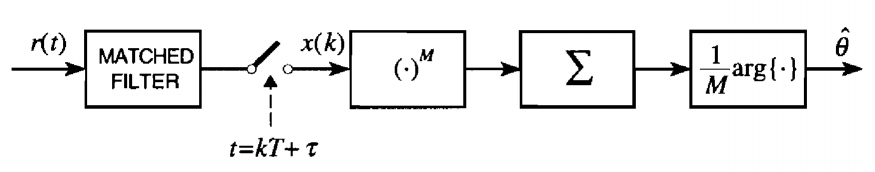
\includegraphics[scale=.3]{figs/m-power.png}
    \end{figure}
\end{frame}

\section{Próxima aula}
\begin{frame}[t]
    \frametitle{Implementação}

    \begin{itemize}
        \item Apesentação de algumas arquiteturas de estimadores de tempo de símbolo.
    \end{itemize}
\end{frame}